% Chapter 4

\chapter{Dataset creation}
\label{Chapter4}

In Chapter~\ref{Chapter3} we finalised our OpenAI environment choice and have a systematic way to generate different configurations of our environments.

The next step is to build up our dataset by solving as many of these configurations as possible with the use of reinforcement learning algorithms.

We justified in previous sections (specifically section~\ref{qlearning} and section~\ref{movationandshortcomings}) how using \emph{model-free} reinforcement learning algorithms will put us in the right direction to achieve the project's goals highlighted in section~\ref{motivation}: improve the transferability of pre-trained models to different configurations, environments, and tasks.

One choice that is left to make before we move on to train models using our randomised environments is what reinforcement learning algorithm we should use.

%----------------------------------------------------------------------------------------

\section{Q-learning on \code{RandomisedFrozenLake}}
We have presented Q-learning in section~\ref{qlearning} as a method that generates a policy by building up a table $Q$ of values corresponding to the expected utility of taking each action at each observable state.

This table $Q$ is represented as a 2D-matrix of size (\code{env.observation\_space.n}, \code{env.action\_space.n}), which in the case of \code{RandomisedFrozenLake} is just a (16x4) matrix.

This is good news. Having a policy that is encoded as a 2-dimensional data structure makes it an obvious input to our Generative Adversarial Network later on in the next chapter. In fact, as we presented in section~\ref{successes}, GANs have proven successful in image synthesis applications, where inputs were images, that is 2D matrices.

The choice of Q-learning as our reinforcement learning technique therefore becomes preferable. Other model-free algorithms like policy search may not have a clear 2D representation in the way the trained parameter set $\theta$ is encoded.

%----------------------------------------------------------------------------------------

\section{Experiment set up}
Before we proceed, we need to be able to record some details about the process of training our data. If our ultimate objective is to benchmark performance of traditional reinforcement learning agains our proposed approach, we need to record running time of our training, and see if that improves at the end. 

Let's encapsulate training of a configuration in an \code{Experiment} class, whose code is shown in listing~\ref{lst:experiment}. An \code{Experiment} is initialised with an OpenAI Gym environment, which in our case is an instance of a \code{RandomisedFrozenLake}, and an integer value \code{num\_episodes}, indicating the number of independent simulations the Q-learning algorithm will be doing. By calling \code{Experiment}'s \code{run()} instance method, we actually start training the model, with $Q$ being updated at each iteration.

The instance variable \code{score} could be used as an evaluation criteria of the effectiveness of our training. It records the average reward the agent achieves for each episode during training.

\code{Experiment} also has a utility method called \code{dumps()} that serialises all this data and allows us to save it on disk.
\\\\
\begin{minipage}{\linewidth}
\lstset{language=Python}
\lstset{frame=lines}
\lstset{caption={\code{Experiment} wrapper class to train one instance of \code{RandomisedFrozenLake}}}
\lstset{label={lst:experiment}}
\lstset{basicstyle=\footnotesize}
\begin{lstlisting}
class Experiment(object):
    def __init__(self, env, num_episodes=10000):
        self.env = env
        self.Q = np.zeros([self.env.observation_space.n, self.env.action_space.n])
        self.num_episodes = num_episodes
        self.score = None
        self.valid_score = None
        self.start = None
        self.end = None
            
    def run(self):
        self.start = datetime.now()
        # ------------------------------------------------------------
        # Run Q-learning algorithm, saving the rewards of each episode
        # ...
        # ...
        # ------------------------------------------------------------
        self.end = datetime.now()
        self.score = sum(rewards)/self.num_episodes
        
    def dumps(self):
        return dumps({'Q': self.Q, 'start': self.start, 'end': self.end, 'score': self.score, 'num_episodes': self.num_episodes})
\end{lstlisting}
\end{minipage}

It's critical to be able to evaluate the quality of the Q-table after training. To do so we just use the optimal policy (that is the policy that picks the action that has the maximum expected utility according to the Q-table) and run if for a certain number of episodes. A validation score could be then defined by the average reward achieved at each episode. Listing \ref{lst:validate_experiment} shows the code to achieve that.

\begin{minipage}{\linewidth}
\lstset{language=Python}
\lstset{frame=lines}
\lstset{caption={Code to validate a trained Q-table}}
\lstset{label={lst:validate_experiment}}
\lstset{basicstyle=\footnotesize}
\begin{lstlisting}
def validate(self):
	rewards = 0
    for i in tqdm(range(num_episodes)):
        while j < 200: # Limit to 200 time steps
            j+=1
            # Choose an action by pick best action from Q-table
            a = np.argmax(Q[s,:])
            
            # Get new state and reward from environment
            s1,r,d,_ = env.step(a)
            rewards += r
            s = s1
            if d == True:
                break
     self.valid_score = rewards / num_episodes
\end{lstlisting}
\end{minipage}

%----------------------------------------------------------------------------------------

\section{Distributed Q-learning}
Now that we formalised our experiment setup, we can run Q-learning on each of the map configurations of our \code{RandomisedFrozenLake}. For the 4x4 grid there are 3,827 possible valid map configurations. It takes an average of 15 seconds to train each Q-learning table on a 2.5 GHz Intel Core i7 processor. On a single machine, it would take around 16 CPU hours to run the whole set of experiments.

To make this step of our pipeline faster and scalable to more data, we decide to set up a distributed processing on a cluster with multiple machines. More precisely, we set up a MapReduce framework \parencite{Dean:2004:MSD:1251254.1251264} implementation running on an Hadoop cluster \parencite{shvachko2010hadoop} of 25 machines.

A MapReduce program is composed of a Map procedure that takes in some (large) input and performs a particular operation whose output is then fed into another Reduce procedure, which outputs the final result. The power of MapReduce is that the framework orchestrates the processing of these procedures by marshalling the distributed servers, running the various tasks in parallel, managing all communications and data transfers between the various parts of the system, and providing for redundancy and fault tolerance.

Figure~\ref{fig:MapReduce} shows the distributed architecture to train multiple Q-learning instances. The input to the system is a list of strings, each representing the map configuration of a \code{RandomisedFrozenLake}, e.g. $"SFHHHFHHHFHHHFFG"$. These inputs are fed into Mapper programs running on different machines. The mapper's task is to initialise the experiment and run Q-learning on the environment. It outputs a key-value pair, where the key is the string that uniquely identifies a map configuration, and the output is the \code{Experiment} object that encapsulates the already trained Q-table. We have yet to assign a validation score to this table we trained, and that's the job of the reducer.

Each experiment's result is then written to an output file by the reducer. Each line will be again a key-value pair, with the map configuration string as key and the \code{Experiment} result dumped in string format. In the following sections, we can just parse and load these results to conduct our further analysis.

While this particular architecture does not make full use of the power of MapReduce (combining, partitioning and sorting), it is an optimal and convenient pipeline to distribute our computations across a cluster of machines, thereby drastically reducing the training time of the whole experiment set.
\begin{figure}
\centering
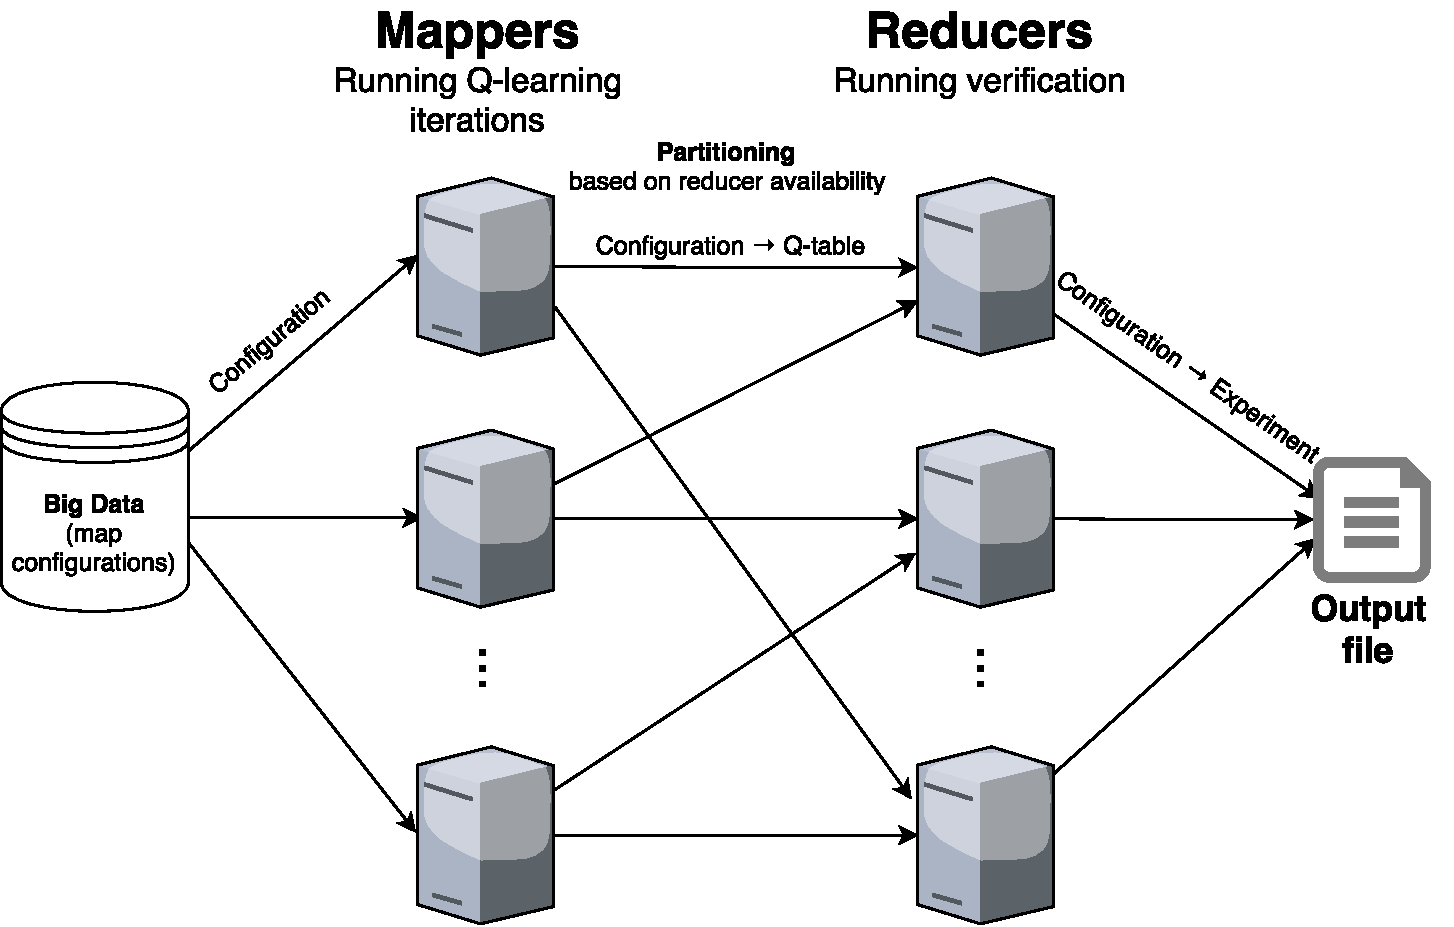
\includegraphics[width=10cm]{Figures/MapReduce}
\caption{Schematic of distributed Q-learning with validation on MapReduce}
\label{fig:MapReduce}
\end{figure}

\section{Analysis of results}
\label{sec:analysisresults}
In this section we report some statistics on the data we just trained. This analysis will be useful when we perform our final benchmarking.

Figure~\ref{fig:Qvalues} shows the average intensity values of the Q-tables in the training subset.

We notice that the utility values in the second and third columns are, in most cases, the highest values at each row. We interpret this as our models favouring, on average, the action of going south (second column) and east (third column) over going west or north.

Indeed, according to the reward system that we described in section~\ref{sec:adjrewardsys}, our trained models will try and reach the goal state with as few actions as possible. This validates why on average, the best actions to make at each state will be going south or going east.
% TODO: Plot rewards plot with std
% TODO: Define acceptable line and when it is achieved

\begin{figure}
\centering
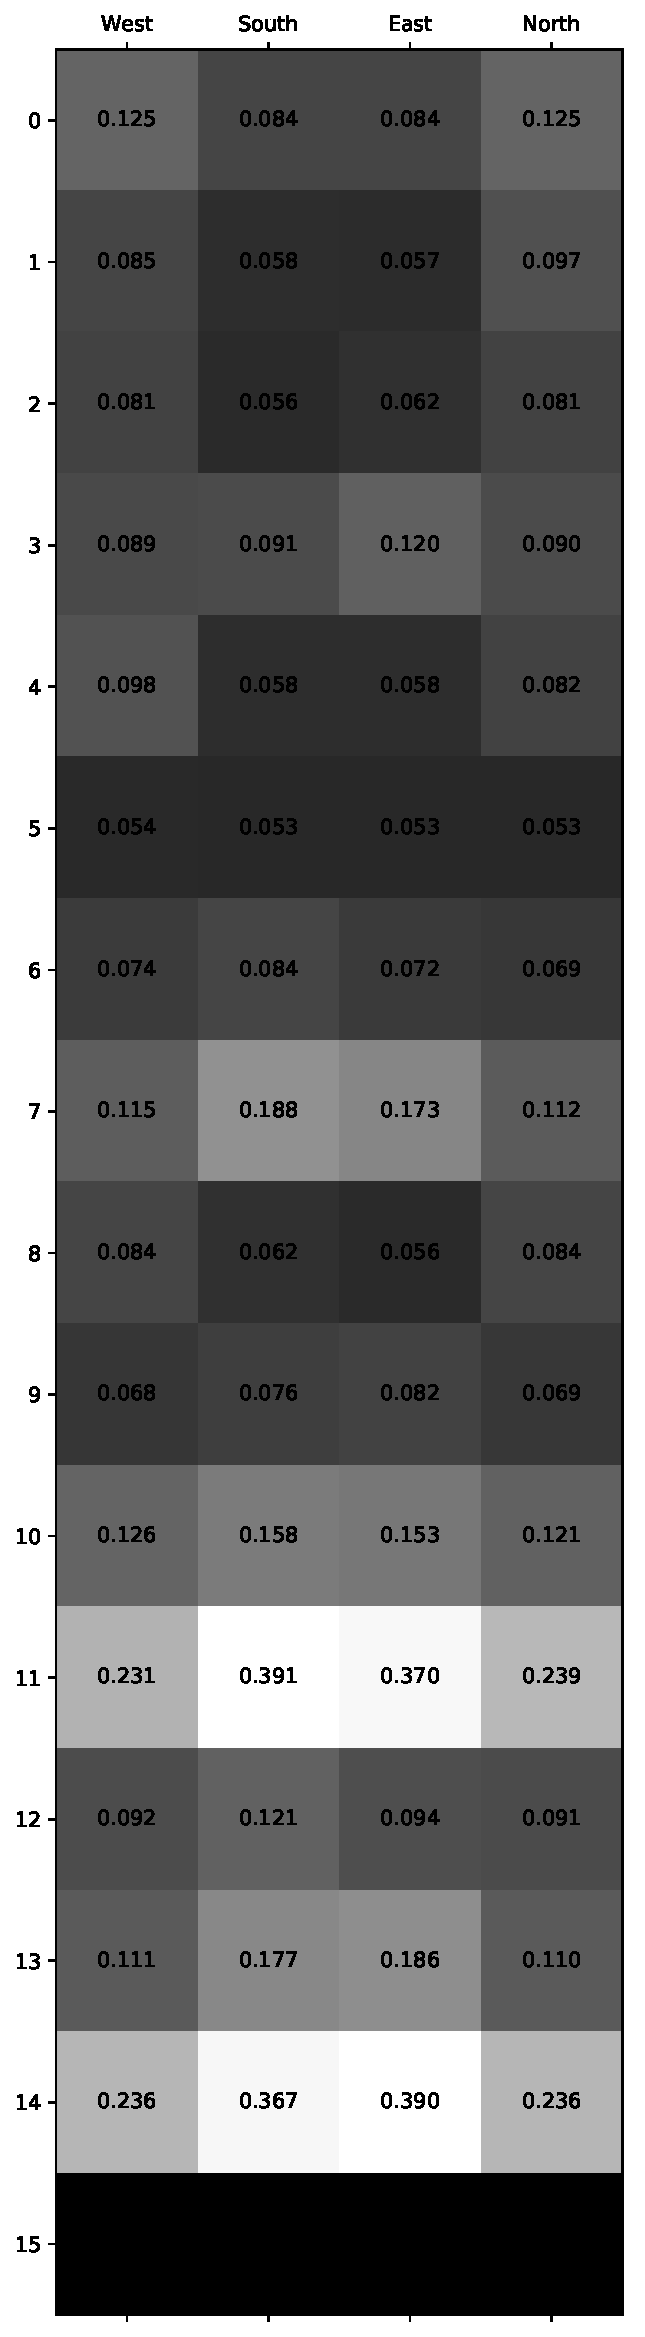
\includegraphics[width=3cm]{Figures/Qtable_mean}
\caption{Average intensity values of the Q-tables in the training subset}
\label{fig:Qvalues}
\end{figure}

\section{Transferable knowledge}
\label{sec:transferableknowledge}
Before proceeding, we need to start a discussion on the type of knowledge that we wish or we expect to be transferred. Having transferred knowledge is what will allow us to speed up training time on unseen tasks.

By using Q-learning to train policies on \code{RandomisedFrozenLake}, we effectively train agents to go from the top-left corner to the bottom-right corner.
In section~\ref{sec:adjrewardsys} we adjusted the reward system so that we reward the agent more if it reaches the goal state in fewer time steps. We implicitly favour actions that go south or east. We have just seen in our results analysis how on average the agent is indeed inclined towards the south-east direction.

In this lays our expectation for transferred knowledge: we hope that this bias towards south-east directions in our distribution of training policies is captured by our Generative Adversarial Network.

If that is the case, we can therefore use this captured knowledge when we train new policies on unseen tasks in the test set of map configurations.

In fact, we expect the training process on new maps to be faster given the knowledge that in order to reach goal state, we should give priority to the south-east direction.

As an intuition, imagine there are two people in a labyrinth, looking for a treasure. The first person knows that they will likely eventually find the treasure if they keep going south-east. The other does not. We expect the first one to reach the treasure much faster. The concept of "going south-east" is the knowledge that we hope to transfer in this task domain.

\section{Task generalisation}
\label{sec:taskgeneralisation}
We explained how we hope to capture transferrable knowledge that is generalisable across similar tasks. We do so by training a GAN using the policy distribution in our training set of policies, and we show this process in the next chapter (Chapter~\ref{Chapter5}).

Before we do that, we ought to talk about how this pipeline generalises on different reinforcement learning task domains. In our work we focused on the Frozen Lake environments, but the ultimate goal of our work is to develop a data pipeline that generalises to most reinforcement learning task domains.

If we hope to transfer knowledge within a domain, one key requirement is that there needs to be transferrable knowledge across these tasks. In our main experiment, we decoded this as being the action of "going south-east". However, with many and more complex domains with a larger action space and observation space, it may not be as trivial to identify such knowledge.

In our work, one of the reasons we chose Frozen Lake environments is that it is straightforward enough to verify that our agents are leveraging and benefitting from previous knowledge.

But in many other applications, we do not expect to be able to even decode the transferred knowledge in words, as we do when we say "going south-east". We will leave that up to the deep neural networks and their inherent statistical foundations to model such behaviour given the distribution we pass it.

By developing our pipeline for transferring knowledge, we provide a generalisable tool that people can use on their own task domains.

%----------------------------------------------------------------------------------------